\documentclass[11pt, a4paper, DIV=12]{scrartcl}

% useful packages 
\usepackage{mathtools}
\usepackage{physics}
\usepackage{graphicx}					  
\graphicspath{{figs/}}



\usepackage{amssymb}
\usepackage{amsmath}
\usepackage{hyperref}
\usepackage[separate-uncertainty=true]{siunitx}
\usepackage{xcolor}
\usepackage{braket} % easy braket notation
\usepackage{enumitem}
\usepackage{booktabs}
\usepackage{here}
\usepackage{cprotect}

\usepackage[backend=biber, sorting=none]{biblatex}
\bibliography{refs.bib}

% \numberwithin{equation}{section}

\title{Applying HMC to the long-range Ising model}
\date{\today}
\author{Harilal Bhattarai \& Marcel Schindler}
\begin{document}
	\maketitle
\section{Introduction}

We already did the one dimensional and two dimensional Ising mode in our previous two exercises. Here we can discuss about long-range Ising model by applying HMC. In long-range nature of interaction, we must renormalize the interaction by N-1 to avoid the solutions blow up. To do so, we can introducing  $ \hat{J}=J/N $.

In this report, we can just include some necessary expression on theory part and in next topic we will illustrate the questions of exercise sheet and analyses the other results. Finally, we can conclude our findings in last part of the report.
\section{Theory}
Here we, also, use the Hamiltonian as:
\begin{equation}
H(s, h)= -J \sum_{<x,y>}s_{x}s_{y} - h \sum_{x}s_{x}
\end{equation}

Here after, we can use $ J > 0 $, therefore the partition function can be written as,
\begin{equation}
Z[J>0]=\int_{-\infty}^{\infty}\frac{d\phi}{\sqrt{2\pi \beta \hat{J}}} e^{-\frac{\phi^2}{2\beta \hat{J}} + \text{N}\log(2\cosh(\beta h \pm \phi))}
\end{equation}

We define the artificial Hamiltonian as,

\begin{equation}
{H(P, \phi)}= \frac{p^2}{2} + \frac{\phi^2}{2\beta \hat{J}} - \text{N}\log 2(\cosh(\beta h + \phi))
\label{equ:ArtificialH}
\end{equation}

\section{Problems Solving and Analysis}
For question one we look at:
\begin{equation}
	\log(Z)=\int_{-\infty}^{+\infty}d\phi\left[-\log(\sqrt{2\pi  J})+\frac{-\phi^2}{2  J}+N\log(2\cosh(\beta h+\phi))\right]
\end{equation}
In this quation we already set $J=\beta\hat{J}$. Now we can take the derivativ:
\begin{equation}
	<m>=\frac{1}{N\beta}\frac{\partial}{\partial h}=\int_{-\infty}^{+\infty}d\phi\underbrace{\tanh(\beta h+\phi)}_{m[\phi]}
\end{equation}
and
\begin{align}
	<\epsilon>=\frac{1}{N}\frac{\partial}{\partial \beta}=&\int_{-\infty}^{+\infty}d\phi\frac{\partial}{\partial J}\frac{\partial J}{\partial \beta}\left(-\log(\sqrt{2\pi J})+\frac{-\phi^2}{2 J}\right)+\frac{\partial}{\partial \beta}N\log(2\cosh(\beta h+\phi))\\
	=& \int_{-\infty}^{+\infty}d\phi \underbrace{-\left(1+\frac{\phi^2}{2 J}+h \tanh(\beta h+\phi)\right)}_{\epsilon[\phi]}\text{.}
\end{align}

To do question two of the exercise sheet, from equation \ref{equ:ArtificialH} we get,

\begin{equation}
\dot{\phi}=\frac{\partial H}{\partial P}= P
\end{equation}
Also,
\begin{equation}
\dot{P}=-\frac{\partial H}{\partial \phi}= \frac{\phi}{\beta \hat{J}} - N \tanh(\beta h+ \phi)
\end{equation}

To do leapfrog algorithm we can follow following steps
\begin{itemize}
	\item Set $(\pi, \phi) = (p_{0}, \phi_{0}) $
	\item At first half, $\phi=\phi +\frac{\epsilon}{2} \pi $\\
	Where, $ \epsilon=\frac{1}{N_{md}} $ split of trajectory upto small pieces $ N_{md} $.
	\item  repeat $ N_{md} - 1$ times\\
	$ \pi=\pi -\epsilon(\frac{\phi}{\beta \hat{J}} - N \tanh (\beta h + \phi)) $\\
	$\phi=\phi +\epsilon \pi $
	\item Last step $ \pi=\pi -\epsilon(\frac{\phi}{\beta \hat{J}} - N \tanh (\beta h + \phi)) $\\
	$\phi=\phi +\frac{\epsilon}{2}\pi $
\item	Set $(P_{f}, \phi_{f}) = (\pi, \phi) $
\end{itemize}
To working with leapfrog algorithm, we have used the HMC algorithm is as follows:
\begin{itemize}
	\item Sample $ P \epsilon[0,1] $
	\item Integrate the EoMs using leapfrog to obtain a trial $ P_{0}, \phi_{0} $
	\item $P_{cc} =min{1 e^{H(P, \phi)- H(P^{\prime}, \phi^{\prime})}} $
	\item Repeat
\end{itemize}
Here by plotting the convergence of leap-frog integrator as a number of integration steps $ N_{md}$ we get a graph \ref{fig:convergence}. In this graph, on the basis of literature, we expect the exponentially decreasing the Hamiltonian with increasing the number of integration steps which we can also see in our plot.
\begin{figure}[H]
	\centering
	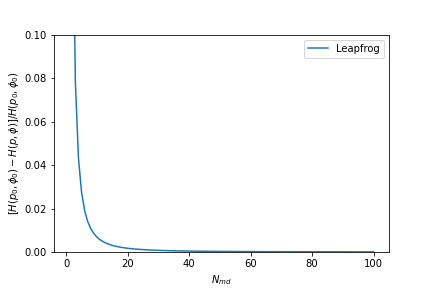
\includegraphics[width=0.8\linewidth]{convergence.png}
	\caption{Convergence of leap-frog integrator as a number of integration steps $ N_{md}$  .}
	\label{fig:convergence}
\end{figure}

To determine the average energy per site, we have set $ h=(\beta h)= 0.5 $ and $ J=(\beta J) \epsilon[0.2, 2.0] $. We had an apcceptance rate for the leapfrog algorithm of $99\%-100\%$. Then, we plotted a graph J vs average energy with different N. From figure \ref{fig:AEnergy} we can see that the average energy decreases more slightly with increasing J at higher number of sites. Also, the numerical value is quite follow the analytic value.
\begin{figure}[H]
	\centering
	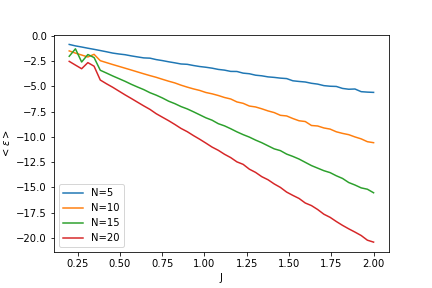
\includegraphics[width=0.6\linewidth]{energy.png}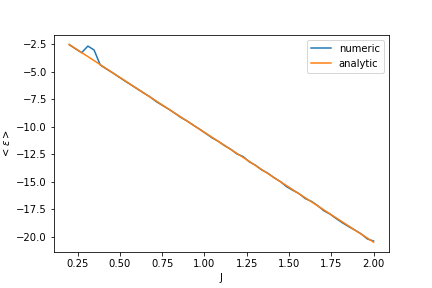
\includegraphics[width=0.6\linewidth]{energy_comparison.png}
	\caption{The average energy per site with different numbers and comparison of its analytic and numerical values.}
	\label{fig:AEnergy}
\end{figure}

To calculate the mean magnetization we have set the value of h and J same as in calculation of average energy. In the output graph \ref{fig:magnetization} between J and average magnetization with different number of sites, we can see that at low J spins are not parallel; however, at higher J all the spins with different site follow parallel paths. We think that in long range Ising model every particles interact each other. Therefore all the spins quickly flow up direction. Also, here, the numerical value has quite good agreement with analytic. 
\begin{figure}[H]
	\centering
	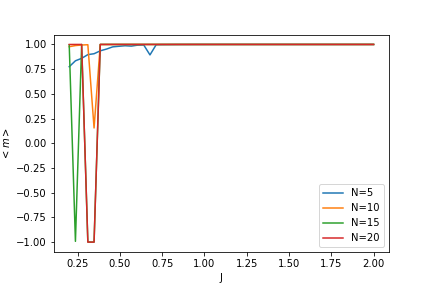
\includegraphics[width=0.6\linewidth]{magnitization.png}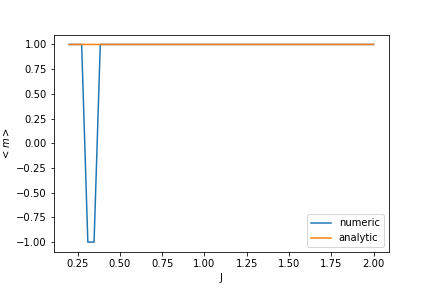
\includegraphics[width=0.6\linewidth]{magnitization_comparision.png}
	\caption{The mean magnetization per site with different numbers and comparison of its analytic and numerical values.}
	\label{fig:magnetization}
\end{figure}
\section{Error-Analysis}
In this section we want to do error-analysis. We did not include errors befor because the graphs become unreadable. So now we want to focus on the eroor. We use the bootsstrap method. Thus we get:
\begin{equation}
	\bar{\mu_{bs}}=\frac{1}{R}\sum_{R}^{b=1}\bar{\mu^b}
\end{equation}
\begin{equation}
\delta\bar{\mu_{bs}}= sd({\bar{\mu^b}})=\sqrt{\frac{1}{R-1}\sum_{R}^{b=1}(\bar{\mu^b}-\bar{\mu_{bs}})^2}
\end{equation}
with $\mu^b$ our samples. After we got $\delta\bar{\mu_{bs}}$ we can do propagation of uncertainty and get:
\begin{equation}
	\delta <m>=\frac{\partial }{\partial \phi} \tanh(h+\phi_bs)\cdot\delta\bar{\phi_{bs}}
\end{equation}
and
\begin{equation}
\delta <\epsilon>=\frac{\partial }{\partial \phi} -\left(1+\frac{\phi^2}{2J}+ \tanh(h+\phi_bs)\right)\cdot\delta\bar{\phi_{bs}}
\end{equation}
We then get the graphs in \ref{fig:error}
\begin{figure}[H]
	\centering
	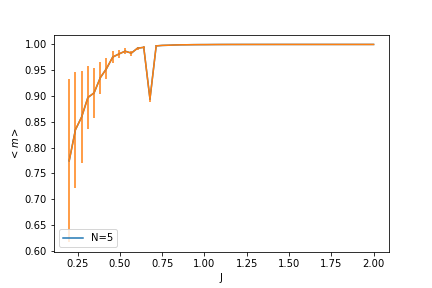
\includegraphics[width=0.6\linewidth]{magnitization_error.png}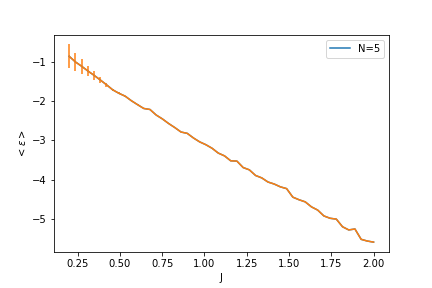
\includegraphics[width=0.6\linewidth]{energy_error.png}
	\caption{Error Analysis for the magnitization and for the energy}
	\label{fig:error}
\end{figure}
We can see that the error is way higher for lower J and with increasing J the error is to small to see it in this graph. So it makes sense that our calculations are better for higher J and not good for lower J because the error in our numerical algorithm is really high.
\section{Conclusion}
To sum up, the convergence of leap-frog integrator as a number of integration steps $ N_{md}$ the difference between the Hamiltonians exponentially decreases the with increasing the number of integration steps. In long range ising model all spins interact each other at low external magnetic field and follow the parallel path at higher  coupling constant. 
\begin{thebibliography}{12}
	\bibitem{exercise-sheet} 
	Thomas Luu, Andreas Nogga, Marcus Petschlies and  Andreas Wirzba, Exercise-sheet, 2020. 
	
	
\end{thebibliography}	
\end{document}	